\documentclass[fontsize = 10pt, paper= a4,twocolumn,column_gap=5zw]{jlreq}

\usepackage[dvipdfmx]{graphicx}
\usepackage{color}
\usepackage{listings}
\usepackage{url}
\definecolor{OliveGreen}{rgb}{0.0,0.6,0.0}
\definecolor{Magenta}{cmyk}{0, 1, 0, 0}
\definecolor{colFunc}{rgb}{1,0.07,0.54}
\definecolor{CadetBlue}{cmyk}{0.62,0.57,0.23,0}
\definecolor{Brown}{cmyk}{0,0.81,1,0.60}
\definecolor{colID}{rgb}{0.63,0.44,0}
\lstset{
language={C},                   %言語の指定
basicstyle={\ttfamily\small},        %書体の指定
backgroundcolor={\color[gray]{.95}}, %背景色と透過度
keywordstyle={\color{blue}},         %キーワード(int, ifなど)の書体指定
commentstyle={\color{OliveGreen}},   %注釈の書体 
stringstyle=\color{Magenta},         %文字列
frame=single,                        %枠縁(leftline,topline,bottomline,lines,trBL,shadowbox, single)
numbers=left,                        %行番号表示
numberstyle={\ttfamily\small},       %行番号の書体指定
breaklines=true,                     %折り返し(自動改行)
breakindent = 10pt,                  %自動改行後のインデント量(デフォルトでは20[pt])	
tabsize=2,                           %タブの大きさ
captionpos=t                         %キャプションの場所(t,b : "tb"ならば上下両方に記載)
}
\renewcommand{\lstlistingname}{図} % キャプション名の指定

\begin{document}

\title{統計分析法 第4週レポート}
\author{202212022 田島瑞起}
\date{2023/10/31}
\maketitle
\section{設問1}
${H_0}$は$A,B,C$の母平均に差がない,${H_1}$は$A,BC$の母平均に差がある。
\section{設問2}
A群の平均体重は60.9742,標準偏差は16.03058。B群の平均体重は59.976,標準偏差は15.94809。
\begin{figure}
    \centering
    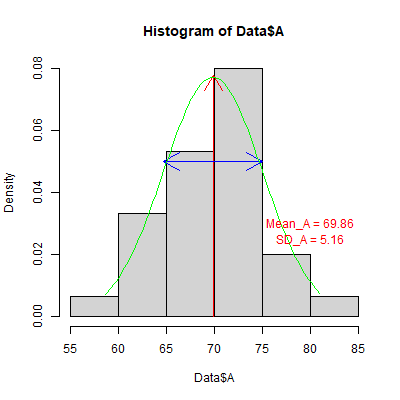
\includegraphics[width=4cm]{4-2-1.png}
\end{figure}

\begin{figure}
    \centering
    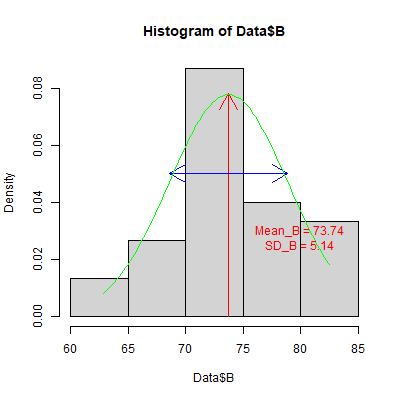
\includegraphics[width=4cm]{4-2-2.png}
\end{figure}

\begin{figure}
    \centering
    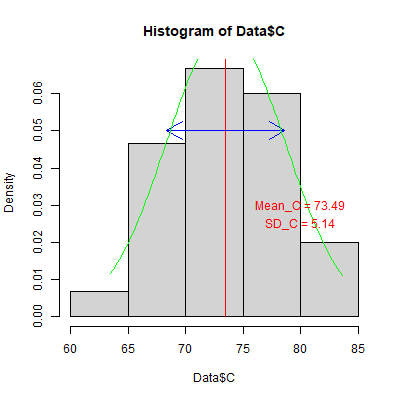
\includegraphics[width=4cm]{4-2-3.png}
\end{figure}

\section{設問3}
$ データ数 = 90$,$自由度 = (2,87) $,$F = 5.351$,$ p = 0.00643$

\section{設問4}
p値が優位水準を満たさないので,${H_0}$は棄却され,A,B,Cの母平均には差があると結論できる。

\section{設問5}
\begin{lstlisting}[basicstyle=\ttfamily\footnotesize, frame=single, caption=s2212022-1.c ,label=s2212022-1.c]
    One-way analysis of means (not assuming equal variances)
    data:  投与データ and 薬の種類
    F = 5.2729, num df = 2, denom df = 58, p-value = 0.00787
\end{lstlisting}


\section{設問6}
$283.4/283.4+2303.9$

\section{ソースコード}
\begin{lstlisting}[basicstyle=\ttfamily\footnotesize, frame=single, caption=s2212022-1.c ,label=s2212022-1.c]
    #課題1
#仮説H0:三群の母平均値は等しい
#帰無仮説H1:三群の母平均値は等しくない

#課題2
Data <- read.table("week4-example.txt",header=TRUE)
Mean_A <- mean(Data$A)
Mean_B <- mean(Data$B)
Mean_C <- mean(Data$C)
Mean_A 
Mean_B
Mean_C
SD_A <- sd(Data$A)
SD_B <- sd(Data$B)
SD_C <- sd(Data$C)
SD_A
SD_B
SD_C

#グラフ描画(A)
png("4-2-1.png", width = 400, height = 400)
hist(Data$A,freq=FALSE)
 # 矢印を描画
arrows(x0 = Mean_A,  y0 = 0.078, x1 = Mean_A, y1 = 0, col = "red", code = 1, angle = 30)
arrows(x0 = Mean_A + SD_A , y0 = 0.05, x1 = Mean_A, y1 = 0.05, col = "blue", code = 1, angle = 30)
arrows(x0 = Mean_A - SD_A,  y0 = 0.05, x1 = Mean_A, y1 = 0.05, col = "blue", code = 1, angle = 30)
# 正規分布で近似した曲線を追加
x <- seq(min(Data$A), max(Data$A), length = 100)
y <- dnorm(x, mean = Mean_A, sd = SD_A)
lines(x, y, col = "green")
text(80,0.030,labels = paste("Mean_A =", round(Mean_A, 2)), col = "red")
text(80,0.025,labels = paste("SD_A =", round(SD_A, 2)), col = "red")
dev.off()

#グラフ描画(B)
png("4-2-2.png", width = 400, height = 400)
hist(Data$B,freq=FALSE)
 # 矢印を描画
arrows(x0 = Mean_B,  y0 = 0.078, x1 = Mean_B, y1 = 0, col = "red", code = 1, angle = 30)
arrows(x0 = Mean_B + SD_B , y0 = 0.05, x1 = Mean_B, y1 = 0.05, col = "blue", code = 1, angle = 30)
arrows(x0 = Mean_B - SD_B,  y0 = 0.05, x1 = Mean_B, y1 = 0.05, col = "blue", code = 1, angle = 30)
# 正規分布で近似した曲線を追加
x <- seq(min(Data$B), max(Data$B), length = 100)
y <- dnorm(x, mean = Mean_B, sd = SD_B)
lines(x, y, col = "green")
text(80,0.030,labels = paste("Mean_B =", round(Mean_B, 2)), col = "red")
text(80,0.025,labels = paste("SD_B =", round(SD_B, 2)), col = "red")
dev.off()

#グラフ描画(C)
png("4-2-3.png", width = 400, height = 400)
hist(Data$C,freq=FALSE)
 # 矢印を描画
arrows(x0 = Mean_C,  y0 = 0.078, x1 = Mean_C, y1 = 0, col = "red", code = 1, angle = 30)
arrows(x0 = Mean_C + SD_C , y0 = 0.05, x1 = Mean_C, y1 = 0.05, col = "blue", code = 1, angle = 30)
arrows(x0 = Mean_C - SD_C,  y0 = 0.05, x1 = Mean_C, y1 = 0.05, col = "blue", code = 1, angle = 30)
# 正規分布で近似した曲線を追加
x <- seq(min(Data$C), max(Data$C), length = 100)
y <- dnorm(x, mean = Mean_C, sd = SD_C)
lines(x, y, col = "green")
text(80,0.030,labels = paste("Mean_C =", round(Mean_C, 2)), col = "red")
text(80,0.025,labels = paste("SD_C =", round(SD_C, 2)), col = "red")
dev.off()

#課題3

#各郡データに分解
Data_A <- Data$A
Data_B <- Data$B 
Data_C <- Data$C

#投与データ(Dataをすべてまとめた変数)を用意する
投与データ <- c(Data_A,Data_B,Data_C)

#薬の種類別ラベルを作成する
薬の種類 <- c(rep("Data_A",30),rep("Data_B",30),rep("Data_C",30))

#要因型ベクトルに分解
薬の種類 <- factor(薬の種類)

#aov関数の実行
summary(aov(投与データ~薬の種類))

#課題4
#p = 0.006となり優位水準を満たさないことから,4群の母平均は等しくないと結論できる

#課題5

oneway.test(投与データ~薬の種類,var.equal=FALSE)
#今回は対応がある場合の分散分析なので
#F=283.4/283.4+2303.9
    \end{lstlisting}

\end{document}